\documentclass[11pt] {article}
\usepackage[a4paper, left=2cm, text={17cm, 24cm}, top=3cm] {geometry}
\usepackage[utf8]{inputenc}
\usepackage[czech]{babel}
\usepackage{times}
\usepackage{graphics}
\usepackage{caption}
\usepackage{float}
\usepackage{array,multirow}
\newcommand{\myuv}[1]{\quotedblbase #1\textquotedblleft}
\setlength{\skip\footins}{10mm plus 2mm}
\usepackage{picture}
\usepackage{pdflscape}
\usepackage{etoolbox}
\patchcmd{\thebibliography}{\section*{\refname}}{}{}{}


\begin{document}
\begin{titlepage}
\begin{center}
\Huge
\textsc{Vysoké učení technické v Brně\\ \vspace{-2mm}
\huge Fakulta informačních technologií} \\
\vspace{\stretch{0.385}}
\LARGE \hspace{-4mm} Počítačové komunikace a sítě\,--\,2. projekt\\[-0.85mm]
\Huge \hspace{0.25mm}  Bandwidth Measurement
\vspace{\stretch{0.615}}
\end{center}
{\Large \today \hfill Jan Vávra}
\end{titlepage}

\tableofcontents
\newpage

\section{Zadání}
Vašim úkolem je:\newline
1. Nastudovat problematiku měření přenosové rychlosti a relevantní informace uvést v projektové dokumentaci. (až 6 bodů)\newline
2. Naprogramovat aplikaci realizující měření přenosové rychlosti mezi dvěma body v síti (až 12 bodů)\newline
3. Provést sadu experimentů pro různé prostředí a toto uvést jakou součást dokumentace (až 2 body)


\section{Teorie}
Přenosová rychlost značí, jaké množství dat si mezi sebou vymění 2 zařřízení na síti. \cite{itslovnik}\newline
Při měření přenosové rychlosti se snažíme vytvořit algoritmus, který bude přesný, rychlý a bez toho, aby ovlivňoval provoz na lince.
Mezi problémy měření přenosové rychlosti patří:\vspace{-5px}
\begin{itemize}
\item Liší se v čase\vspace{-5px}
\item Projevuje se vysokou rozmanitostí \cite{end-to-end}
\end{itemize}
Jedna z možností měření rychlosti je, že testovací zařízení bude zároveň zasílat zprávy testovanému zařízení a příjmat zprávy od testovaného zařízení. Díky tomuto řešení může testovací zařízení snadno zjistit, kolik packetů bylo posláno a kolik jich bylo přijato.\newline
\begin{center}
\hspace{100px}\scalebox{0.5}{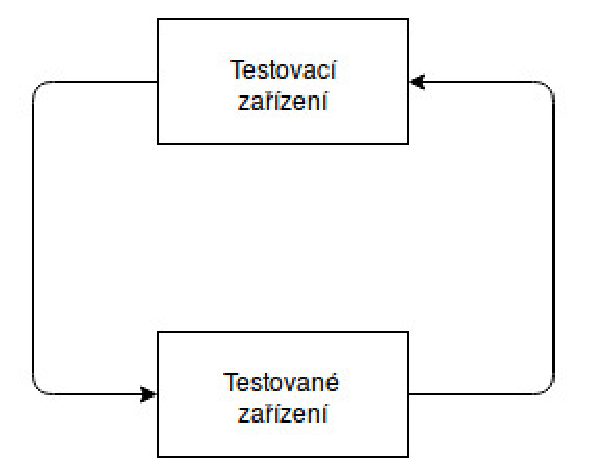
\includegraphics{dut1.eps}}\newline
\end{center} 
Další z možností je oddělit zasílání a příjímání zpráv,ale je třeba zajistit,aby odesílatel a příjemce byl vzdáleně kontrolován jedním počítačem, jinak je toto řešení nemožné. \cite{rfc}
\begin{center}
\hspace{75px}\scalebox{0.5}{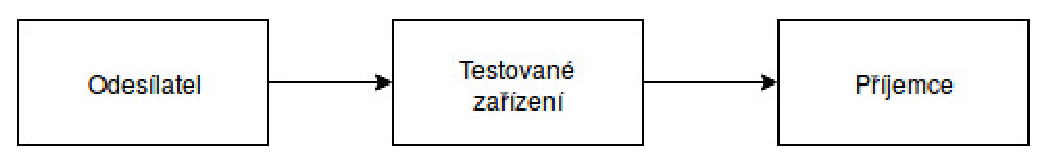
\includegraphics{dut2.eps}}\newline
\end{center}
\newpage
\section{Implementace}
\subsection{Implementace reflektoru}
Reflektor po spuštění čeká na prvotní zprávu od měřáku(CONNECT\#\emph{velikost\_sondy}), která obsahuje velikost sondy,kterou bude dostávat. Po obdržení realokuje velikost bufferu pro zprávu, zanoří se do cyklu reflektování a reflektuje dokud neobdrží zprávu o ukončení měření (END). Poté se vrátí v hlavní smyčce na začátek a čeká na další měření. Reflektor se ukončuje pomocí CTRL\-C.

\subsection{Implementace měřáku}
Měřák na svém začátku zašle zprávu reflektoru (CONNECT\#\emph{velikost\_sondy}), aby ho informoval o velikosti sondy, kterou bude zasílat. Následně čeká na odpověď od reflektoru(CONNECT), jestli se úspěšně připojil. V případě neobdržení zprávy měřák končí s neúspěchem.\newline
Pokud úspěšně obdrží odpověď, měřák přejde na testování připojení mezi měřákem a reflektorem. Měřák se rozdělí na dva procesy, odesílatele a příjemce. Po dobu 2 sekund posílá sondy na měřák a následně počítá, které úspěšně přijal. Pokud je počet přijatých ku odeslaným větší než 10, měřák zvedne čas spánku (v mocninách 2) a zkouší znovu. Pokud obdrží 3 sekvence po sobě v pořádku (připouští se malá ztrátovost) měřák se přesune na měření upload rychlosti.\newline
Čas získaný v argumentu je rozkouskován na 10 intervalů, na kterých se následně měří rychlost. Během měření jeden proces odesílá zprávy s jejich časem poslání, druhý proces ukládá přijaté zprávy do fronty spolu s jejich časem příjetí. Po měření se zkontroluje jaký je rozdíl mezi přijatýmy a odeslanýmy zprávami.
Pokud se rovnají čas spánku je snížen o 5\%, pokud se nerovnají čas spánku je zvednut o 10\%.
Po ukončení měření se zašle zpráva reflektoru o ukončení měření(END), spočítají výsledky a vypíšou se uživateli.


\section{Ukázka měření}
\subsection{Měření loclahost}
\scalebox{0.5}{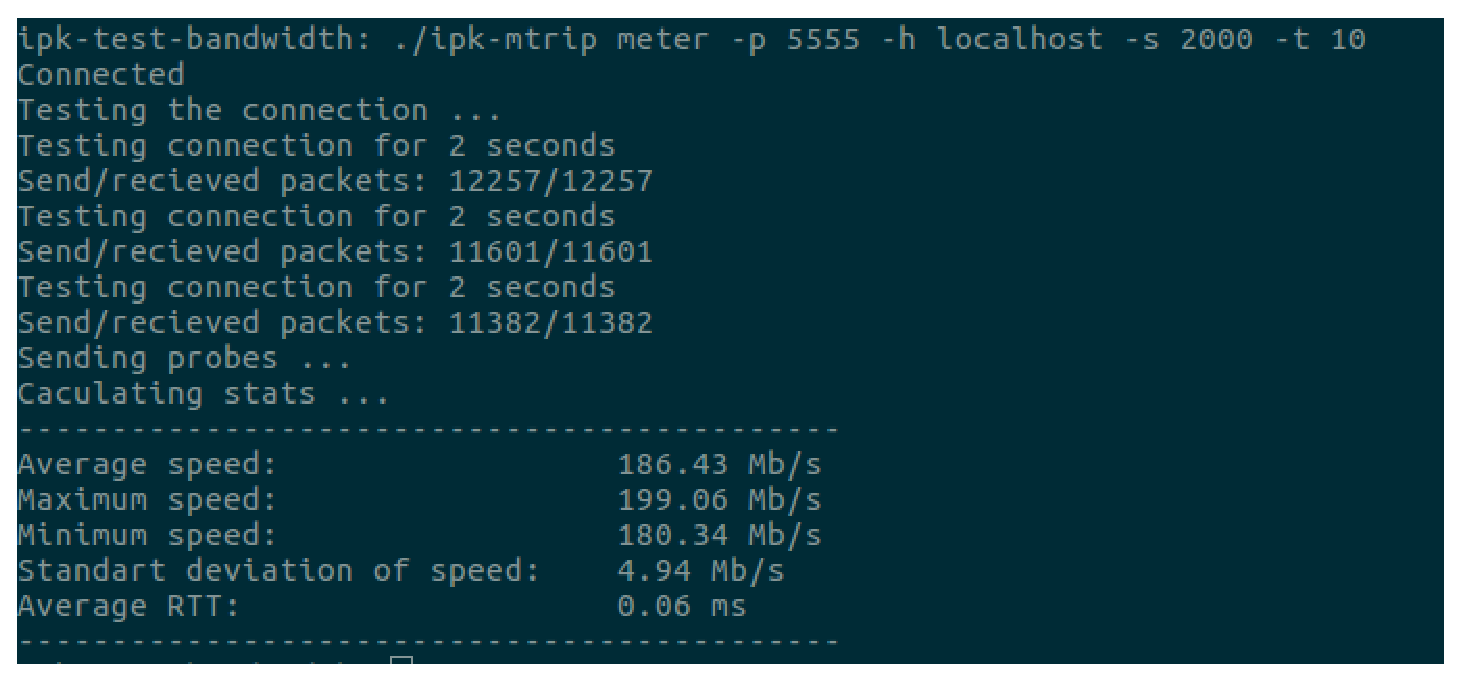
\includegraphics{Measurement1.eps}}\newline
\subsection{Měření loclahost s umělým delay}
\scalebox{0.5}{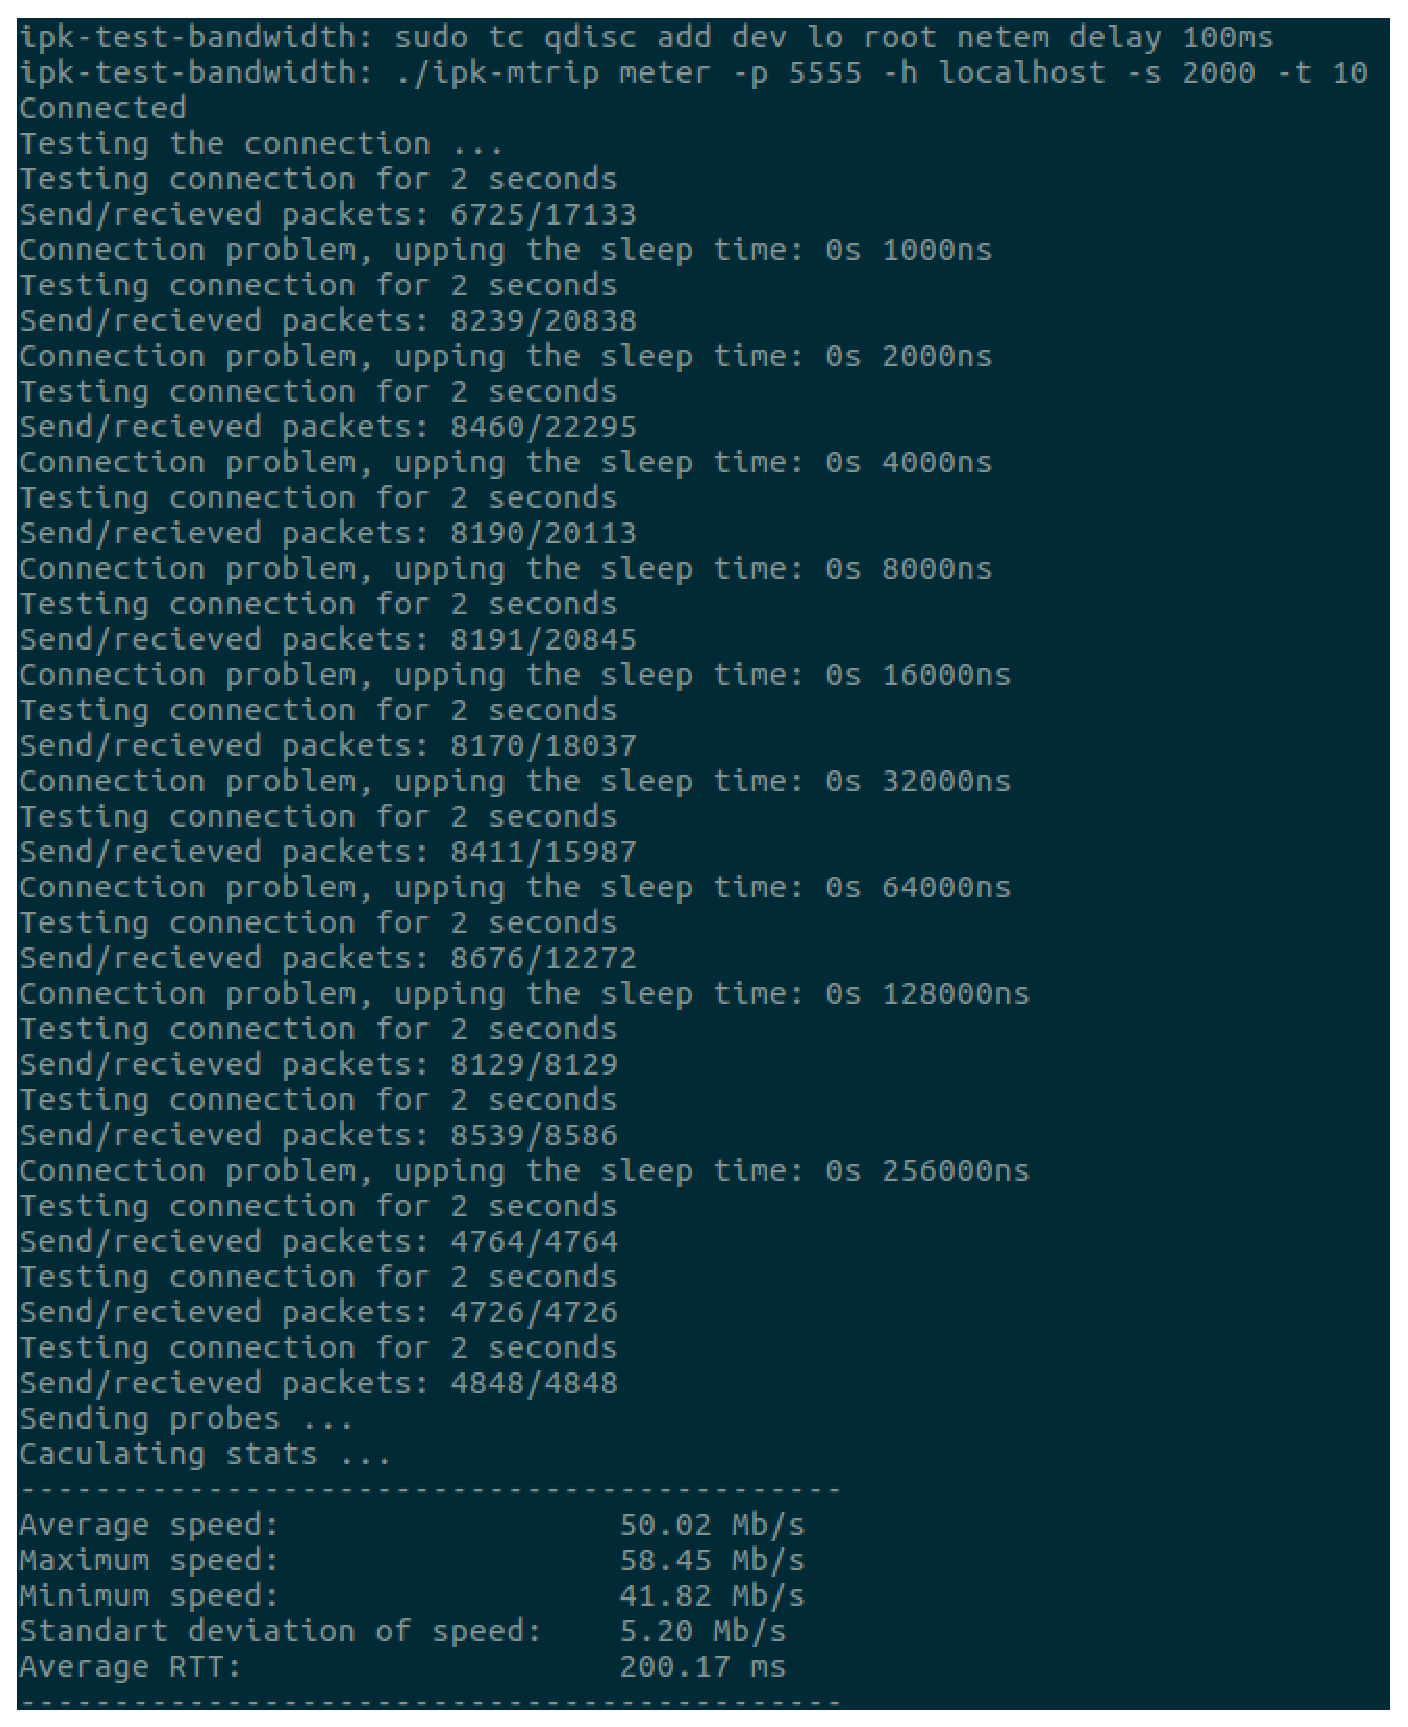
\includegraphics{Measurement2.eps}}\newline
\subsection{Měření loclahost s největší možnou velikostí packetu}
\scalebox{0.5}{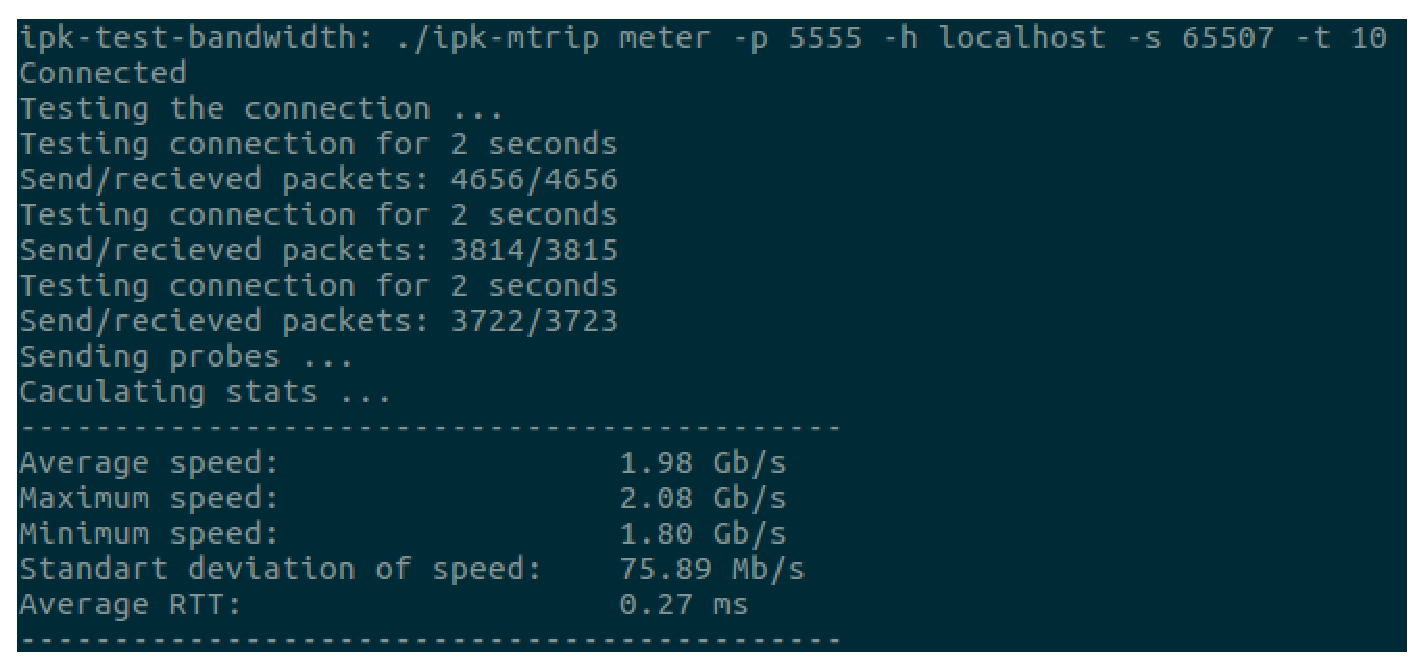
\includegraphics{Measurement3.eps}}\newline
\subsection{Měření na merlina}
\scalebox{0.5}{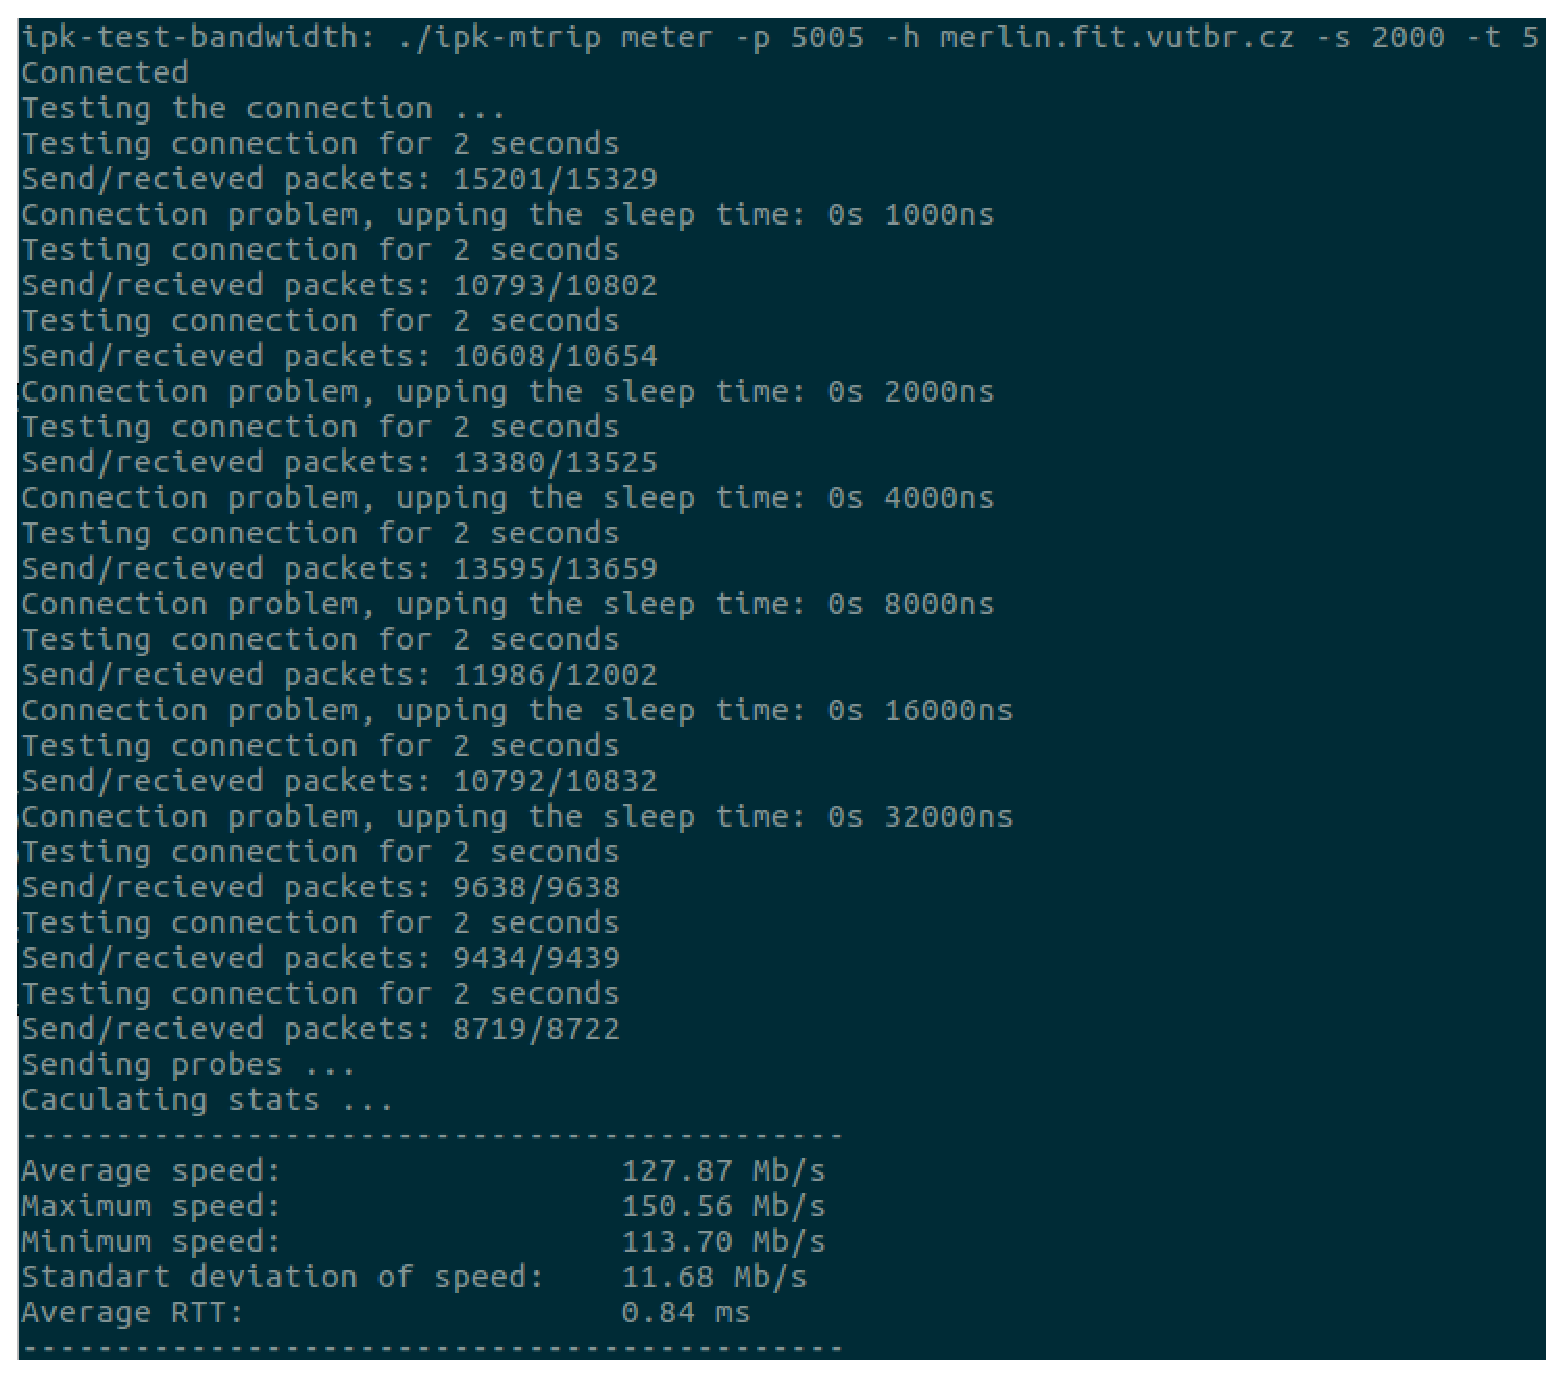
\includegraphics{Measurement4.eps}}\newline
\subsection{Měření na merlina s největší možnou velikostí packetu }
\scalebox{0.5}{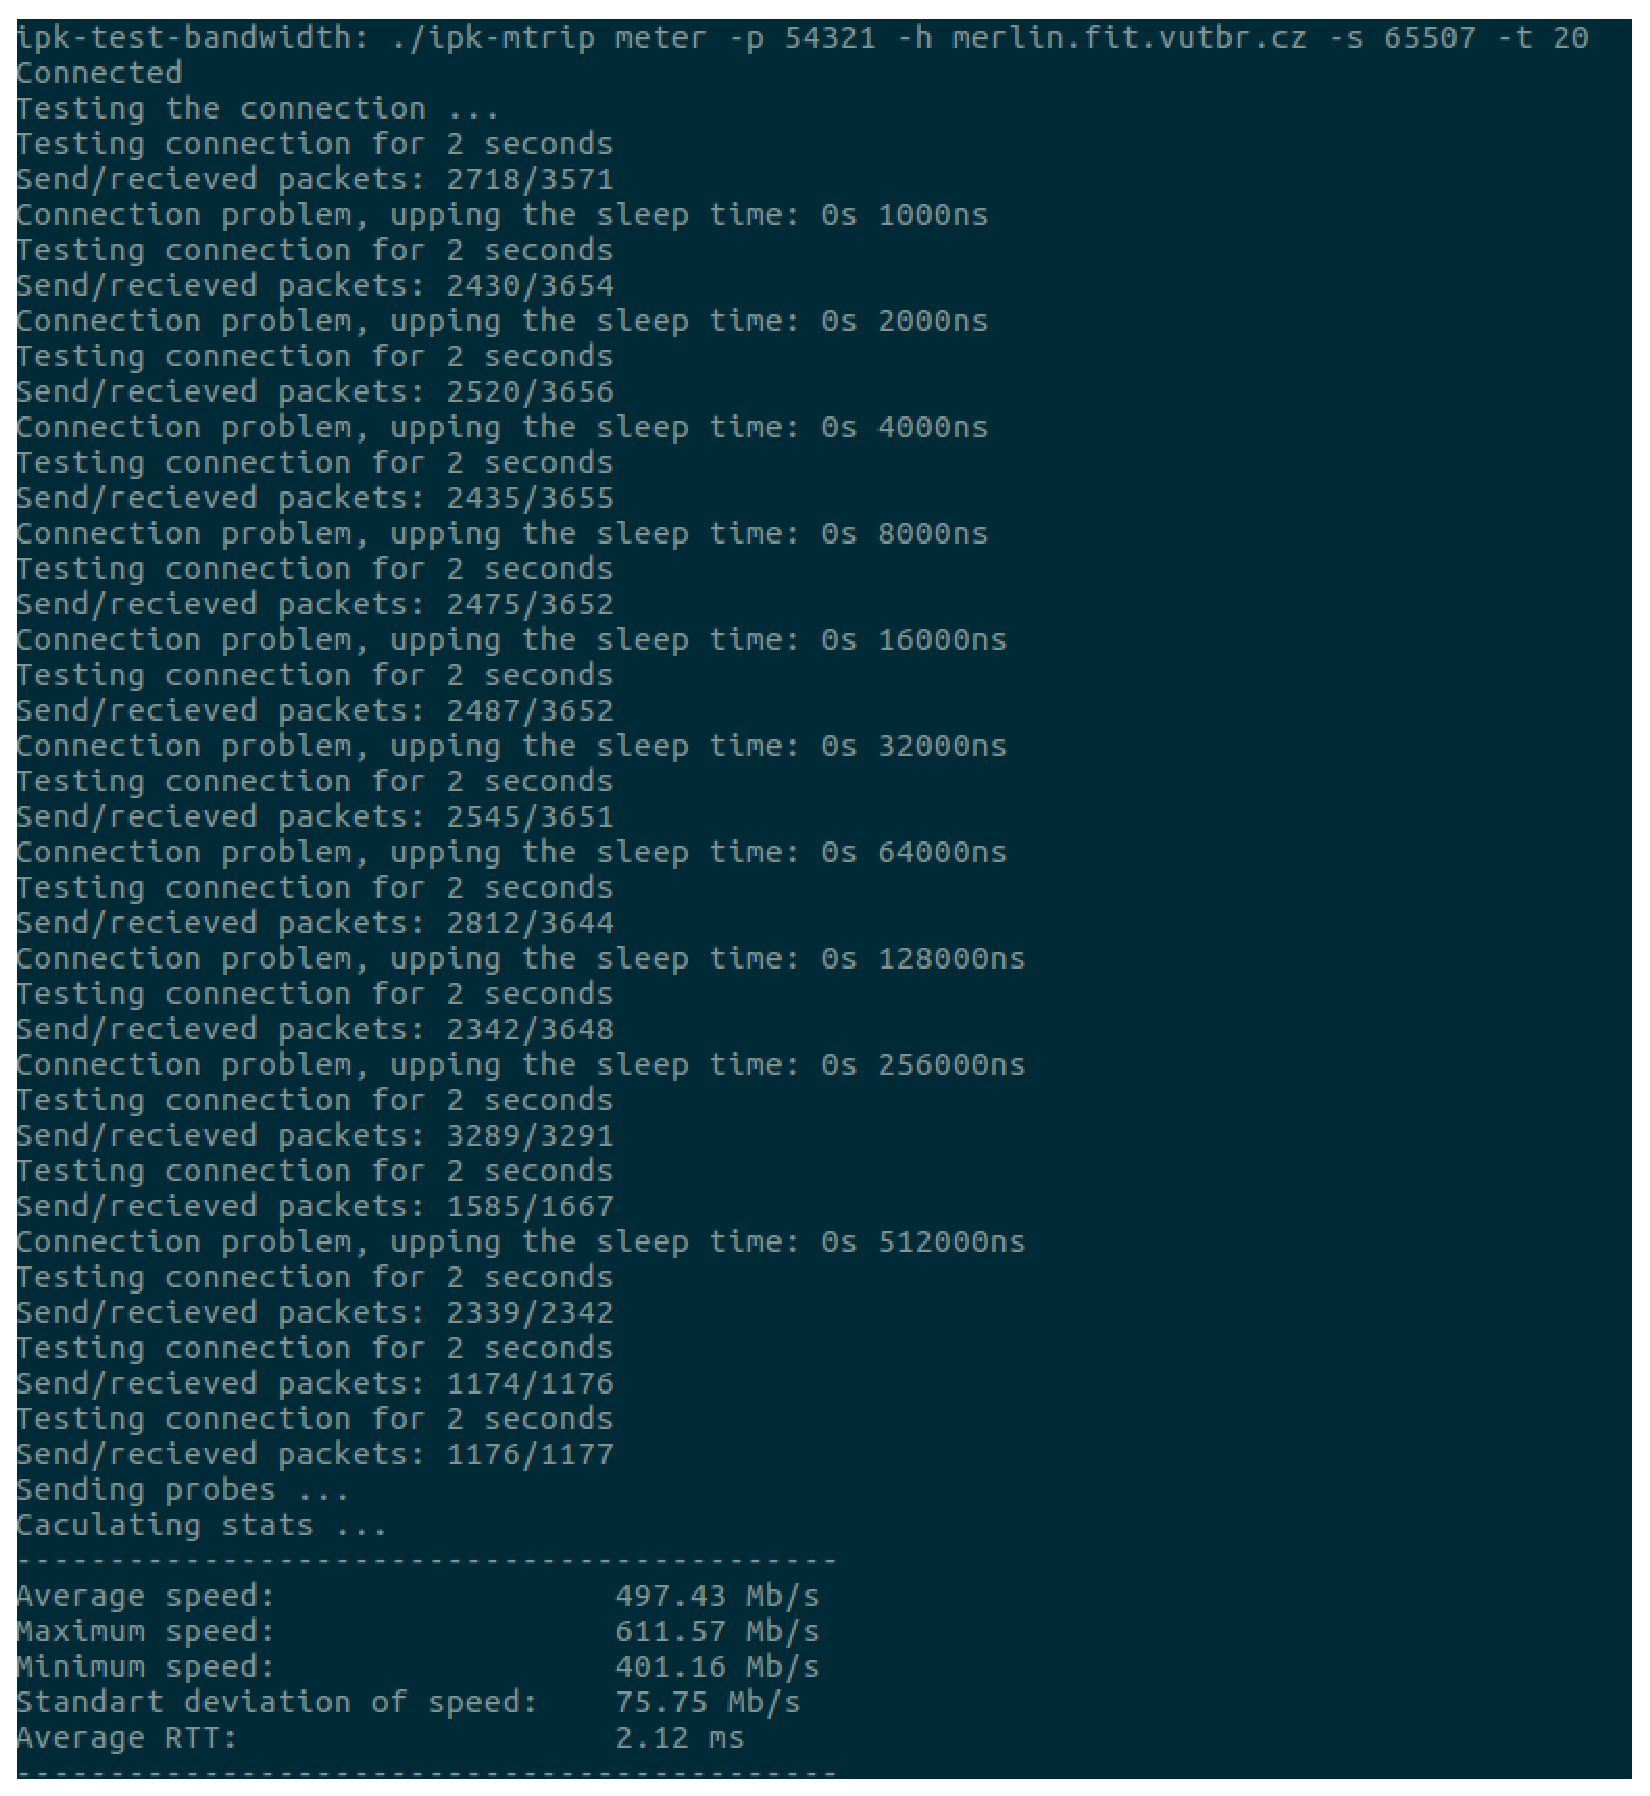
\includegraphics{Measurement6.eps}}\newline
\newpage
\section{Literatura}
\begin{thebibliography}{9}

\bibitem{itslovnik}
  \emph{Přenosová rychlost} [online]. 
  [cit. 2018-04-08]. 
  Dostupné z: https://it-slovnik.cz/pojem/prenosova-rychlost

\bibitem{end-to-end}
	M. Jain and C. Dovrolis, \emph{End-to-end available bandwidth: measurement methodology, dynamics, and relation with TCP throughput}, in IEEE/ACM Transactions on Networking, vol. 11, no. 4, pp. 537-549, Aug. 2003.
DOI: 10.1109/TNET.2003.815304

\bibitem{rfc}
	Bradner, S. and J. McQuaid, \emph{Benchmarking Methodology for Network Interconnect Devices}, RFC 2544, DOI 10.17487/RFC2544, March 1999, Dostupné z: https://www.rfc-editor.org/info/rfc2544.
\end{thebibliography}
\end{document}

